\documentclass{article}
\usepackage[margin=1in]{geometry}
\usepackage{amsmath,amsthm,amssymb}
\usepackage{bbm,enumerate,mathtools}
\usepackage{tikz,pgfplots}
\usepackage{chessboard}
\usepackage[hidelinks]{hyperref}
\usepackage{multicol} % Problem 35

\newenvironment{question}{\begin{trivlist}\item[\textbf{Question.}]}{\end{trivlist}}
\newenvironment{note}{\begin{trivlist}\item[\textbf{Note.}]}{\end{trivlist}}
\newenvironment{references}{\begin{trivlist}\item[\textbf{References.}]}{\end{trivlist}}
\newenvironment{related}{\begin{trivlist}\item[\textbf{Related.}]\end{trivlist}\begin{enumerate}}{\end{enumerate}}


\begin{document}
  Consider a $2$-coloring of a triangular grid of length $\ell$. Then label each
  cell with its greatest number of neighbors of one color.\\\vspace{0.5cm}
\begin{figure}[!h]
  \centering
  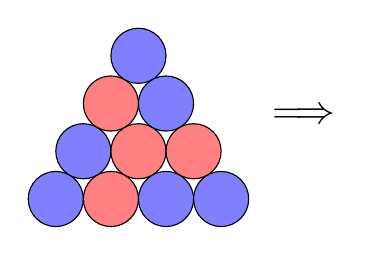
\begin{tikzpicture}[scale=0.7]
    \foreach \x/\y/\c in {
      0/0/blue, 0/1/blue, 0/2/red,  0/3/blue,
      1/0/red,  1/1/red,  1/2/blue,
      2/0/blue, 2/1/red,
      3/0/blue} {
      \draw[fill=\c!50] (\x + 0.5 * \y, {\y * sqrt(3)/2}) circle (0.5cm);
    }
    \node at (4.5, 1.5) {\Large $\Longrightarrow$};
  \end{tikzpicture}
  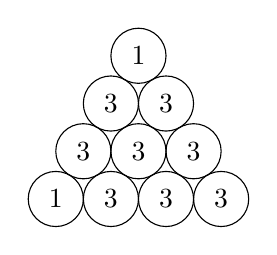
\begin{tikzpicture}[scale=0.7]
    \foreach \x/\y/\c in {
      0/0/1, 0/1/3, 0/2/3,  0/3/1,
      1/0/3,  1/1/3,  1/2/3,
      2/0/3, 2/1/3,
      3/0/3} {
      \draw (\x + 0.5 * \y, {\y * sqrt(3)/2}) circle (0.5cm) node {\c};
    }
  \end{tikzpicture}

  \caption{
    The second cell (reading top to bottom and left to right) is labeled with a
    $\max(3, 1) = 3$ because it has $3$ blue neighbors and $1$ red neighbor.
  }
\end{figure}

\begin{question}
  How many colorings exist of a length $\ell$ triangle such that the maximum
  label is $3$?
\end{question}
\begin{related}
  \item If the ``number triangle'' is summed for each coloring, which coloring
    has the smallest sum?
  \item How does this generalize for a $k$-coloring?
  \item How does this generalize to a $n \times m$ square grid where
    horizontal-vertical connections are counted? Diagonal connections? Both?
  \item How does this generalize to a tetrahedron, torus, M\"obius strip,
    cylinder, or cube?
  \item How many colorings exist of a length $\ell$ triangle such that the maximum
    label is $4$ or $5$?
\end{related}
\end{document}
